\section{Одновыборочные задачи}

На рис. 8.1 представлена схематическая диаграмма метода бутстрепа применительно к одновыборочным задачам. Слева --- реальный мир, где неизвестное распределение $F$ порождает наблюдаемые данные $\textbf{x} = (x_1, x_2, \ldots, x_n)$ путем генерации случайной выборки. Мы вычислили интересующую статистику из $\textbf{x}, \hat{\theta} = s(\textbf{x})$, и хотим узнать что-нибудь о статистическом поведении $\hat{\theta}$, возможно, о его стандартной ошибке $\text{se}_F (\hat{\theta})$.

\noindent
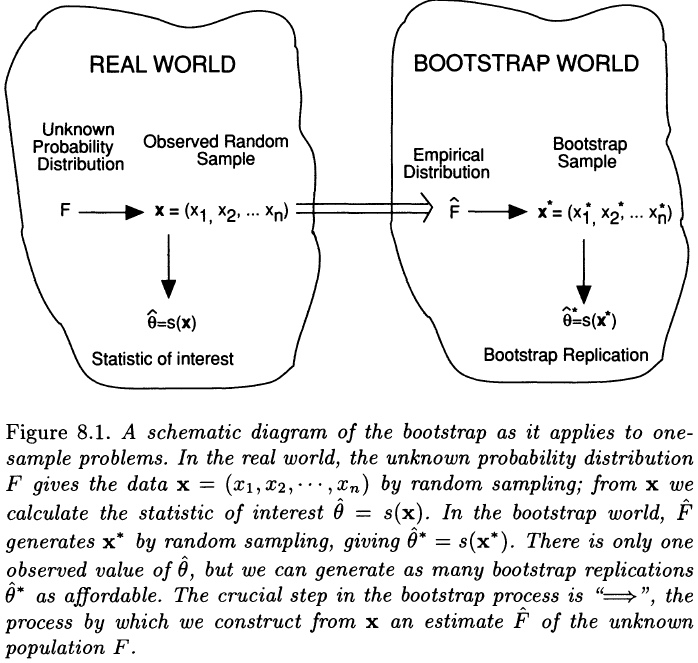
\includegraphics[width=\linewidth]{8/f81}
\newline

В правой части рисунка находится мир бутстрепа, если использовать терминологию Дэвида Фридмана. В мире бутстрепа эмпирическое распределение $\hat{F}$ порождает бутстреп выборки $\textbf{x}^* = (x_1^*, x_2^*, \ldots, x_n^*)$ путем генерации случайной выборки, на основе которой мы вычисляем бутстреп репликации интересующей статистики, $\hat{\theta}^* = s(\textbf{x}^*)$. Большим преимуществом мира бутстрепа является то, что мы можем вычислить столько репликаций $\hat{\theta}^*$, сколько захотим, или, по крайней мере, столько, сколько мы можем себе позволить. Это позволяет нам делать вероятностные вычисления напрямую, например, используя наблюдаемую изменчивость $\hat{\theta}^*$ для оценки ненаблюдаемой величины $\text{se}_F(\hat{\theta})$.

Двойная стрелка на рис. 8.1 указывает на вычисление $\hat{F}$ из $F$. По идее, это решающий шаг в процессе бутстрепа, даже несмотря на то, что он прост в вычислительном отношении. Любая другая часть картины бутстрепа определяется аналогично: $F$ порождает $\textbf{x}$ путем генерации случайной выборки, поэтому $\hat{F}$ порождает $\textbf{x}^*$ путем генерации случайной выборки; $\hat{\theta}$ получается из $\textbf{x}$ через функцию $s(\textbf{x})$, поэтому $\hat{\theta}^*$ получается из $\textbf{x}^*$ таким же образом. Расчеты бутстрепа для более сложных вероятностных механизмов оказываются простыми, если мы знаем, как реализовать процесс, обозначенный двойной стрелкой --- оценку всего вероятностного механизма на основе данных. К счастью, это легко сделать для всех распространенных структур данных.

Чтобы облегчить изучение более сложных структур данных, мы будем использовать обозначение
\begin{equation}
	P \to \textbf{x},
\end{equation}
чтобы указать, что неизвестная \textit{вероятностная модель} $P$ породила наблюдаемый набор данных $\textbf{x}$.